\chapter{Lyapunov Functions and the Limits of Descent}\label{chap:lyapunov}

The heuristic that has accompanied the $3x+1$ problem since the work of
Terras\index{Terras, R.}~\cite{terras1976}, Crandall\index{Crandall, R. E.}~\cite{crandall1978} and Lagarias\index{Lagarias, J. C.} and Weiss\index{Weiss, A.}~\cite{lagarias1992} is, at
bottom, a statement about a potential function.  The quantity $\log x$ goes
down on average along a Collatz orbit, and a quantity that goes down on
average, and cannot go below zero, ought eventually to reach its floor.  In dynamical systems and optimization this is the language of Lyapunov functions\index{Lyapunov function}, and the purpose of this chapter is to take that language
seriously: to say precisely what a Lyapunov certificate\index{certificate} for the Collatz map
would be, to prove what can be proved about the natural candidates, and to
show, with complete proofs, why every candidate of the most natural kind must
fail.

The chapter has a positive half and a negative half.  The positive half is the
stride descent theorem, \cref{thm:stride}, which describes exactly when a
single Syracuse stride decreases $\log x$ and by how much, together with an
exact analysis of two stride compositions.  The negative half consists of
three obstructions.  No single stride Lyapunov function that is monotone in
the size of $x$ can certify descent (\cref{thm:nolyapunov}); no monotone certificate
built from any fixed number $J$ of strides can do so either, because ascending
strides can be chained to arbitrary length
(\cref{prop:ch4:chain,cor:ch4:multistride}); and the natural majorization\index{majorization}
minimization construction for $\log$ yields only a tangent line bound\index{MM algorithm},
which holds for any next iterate and whose surrogate drifts upward in the model
(\cref{prop:mmdescent,prop:mmfails}).  The last
obstruction has a clean explanation in terms of the martingale\index{martingale} duality of
\cref{chap:stochastic}, and it points to the family of power majorizers, which
repair the drift\index{drift} but not the pointwise failure.

Throughout, $S$ denotes the Syracuse map\index{Syracuse map} of \cref{def:maps},
$S(x)=(3x+1)/2^{k}$ with $k=\vt(3x+1)$, acting on odd positive integers, and
$T_0$ and $T$ denote the standard and accelerated map\index{accelerated map}s.

\section{Lyapunov functions for discrete dynamics}\label{sec:ch4:discrete}

Let $f:X\to X$ be a map on a set $X$ and let $A\subset X$ be a target set.
Lyapunov\index{Lyapunov, A. M.}'s idea, set out in his 1892 thesis on the stability of motion~\cite{lyapunov1992} and
carried into the discrete setting by LaSalle\index{LaSalle, J. P.} and others~\cite{lasalle1986}, is
to certify that orbits approach $A$ without computing them, by exhibiting a
scalar function that decreases along every orbit outside $A$.

\begin{definition}[Lyapunov certificate]\label{def:ch4:lyap}
A function $V:X\to\R$ is a \emph{Lyapunov function\index{Lyapunov function}} for $(f,A)$ if
$V(f(x))\le V(x)$ for every $x\notin A$.  It is a \emph{strict} Lyapunov
function if $V(f(x))<V(x)$ for every $x\notin A$, and a \emph{strong} (or
geometric) Lyapunov function if $V>0$ on $X\setminus A$ and there is a
constant $\rho<1$ with $V(f(x))\le\rho\,V(x)$ for every $x\notin A$.
\end{definition}

On a continuum, a strict Lyapunov function need not drive orbits into $A$;
the decrease can become arbitrarily small, and LaSalle's invariance principle
is the tool that identifies where such orbits accumulate~\cite{lasalle1986}.
The situation is simpler when $V$ takes values in the nonnegative integers, or decreases by at least a fixed amount, because a strictly decreasing sequence of nonnegative integers, or a sequence of reals bounded below that decreases by at least a fixed amount at each step, must stop.

\begin{proposition}[Discrete Lyapunov criterion]\label{prop:ch4:discrete}
Let $f:X\to X$ and $A\subset X$.  Suppose that either
\begin{enumerate}[label=(\roman*)]
\item $V$ takes values in $\N\cup\{0\}$ and $V(f(x))<V(x)$ for $x\notin A$; or
\item $V\ge0$ and there is $\varepsilon>0$ with $V(f(x))\le V(x)-\varepsilon$
  for $x\notin A$; or
\item $V\ge c>0$ on $X\setminus A$ and $V(f(x))\le\rho V(x)$ for $x\notin A$,
  with $\rho<1$.
\end{enumerate}
Then every orbit of $f$ enters $A$.  In case (ii) it does so within
$V(x)/\varepsilon$ steps, and in case (iii) within
$1+\log(V(x)/c)/\log(1/\rho)$ steps.
\end{proposition}

\begin{proof}
Suppose that the first $n\ge1$ points $x,f(x),\dots,f^{(n-1)}(x)$ of the orbit lie outside $A$. In case (i) $V$ takes the $n+1$ distinct values $V(x)>V(f(x))>\dots>V(f^{(n)}(x))$, all in $\{0,1,\dots,V(x)\}$, so $n\le V(x)$. In case (ii), $0\le V(f^{(n)}(x))\le V(x)-n\varepsilon$, so $n\le V(x)/\varepsilon$. In case (iii) the bound $V\ge c$ is known only outside $A$, so $c\le V(f^{(n-1)}(x))\le\rho^{n-1}V(x)$ and $n\le1+\log(V(x)/c)/\log(1/\rho)$. In each case $n$ is bounded, so the orbit enters $A$, and the number of steps it takes obeys the stated bound.
\end{proof}

The Collatz conjecture\index{Collatz conjecture} is equivalent to the existence of such a certificate\index{certificate},
and this is worth recording at the outset because it shows that existence is
not the issue.

\begin{remark}[Certificates exist if and only if the conjecture holds]
\label{rem:ch4:exists}
Let $X$ be the odd positive integers, $f=S$ and $A=\{1\}$.  If every Syracuse
orbit reaches $1$, let $\sigma_S(x)$ be the number of strides it takes.  Then
$V=\sigma_S$ satisfies case (i) of \cref{prop:ch4:discrete}, since
$\sigma_S(S(x))=\sigma_S(x)-1$, and $W=2^{\sigma_S}$ satisfies case (iii) with
$c=2$ and $\rho=\tfrac12$.  Conversely any certificate of the kind in
\cref{prop:ch4:discrete} proves that every orbit reaches $1$.  The difficulty
is therefore never whether a Lyapunov function exists but whether one can be
written down without knowing the answer.  The functions $\sigma_S$ and
$2^{\sigma_S}$ are wildly irregular in $x$; the candidates one can actually
analyse are smooth increasing functions of the size of $x$, and those are the ones this
chapter shows to be inadequate.
\end{remark}

\section[Stochastic Lyapunov functions and Foster's criterion]{Stochastic Lyapunov functions and\\ Foster's criterion}
\label{sec:ch4:foster}

The stochastic analogue of a Lyapunov function\index{Lyapunov function} replaces pointwise decrease by
decrease in conditional expectation.  The idea goes back to
Foster\index{Foster, F. G.}~\cite{foster1953}, who used it to decide positive recurrence of
countable Markov chains arising in queueing, and it is the organizing
principle of the monograph of Meyn\index{Meyn, S. P.} and Tweedie\index{Tweedie, R. L.}~\cite{meyn1993}, where it
appears in many forms under the name of drift\index{drift} conditions.

\begin{theorem}[Foster's criterion]\label{thm:ch4:foster}
Let $(X_n)$ be an irreducible Markov chain on a countable set $E$, let
$V:E\to[0,\infty)$, let $C\subset E$ be finite and $\varepsilon>0$.  Suppose
\begin{align*}
  \E\bigl[V(X_1)\mid X_0=x\bigr]&\le V(x)-\varepsilon &&(x\notin C),\\
  \E\bigl[V(X_1)\mid X_0=x\bigr]&<\infty &&(x\in C).
\end{align*}
Then the chain is positive recurrent.  Moreover, if $\tau_C$ is the hitting
time of $C$, then $\E_x[\tau_C]\le V(x)/\varepsilon$ for every $x\notin C$.
\end{theorem}

The positive recurrence statement is Foster's theorem~\cite{foster1953}; see
Meyn and Tweedie~\cite{meyn1993} for the general theory.  The hitting time
bound is elementary and we prove it, because it is exactly the stochastic
counterpart of case (ii) of \cref{prop:ch4:discrete}.

\begin{proof}[Proof of the hitting time bound]
Fix $x\notin C$ and put $M_n=V(X_{n\wedge\tau_C})+\varepsilon\,(n\wedge\tau_C)$.
On the event $\{\tau_C>n\}$ the drift condition gives
$\E[M_{n+1}\mid\Filt_n]\le V(X_n)-\varepsilon+\varepsilon(n+1)=M_n$, and on
$\{\tau_C\le n\}$ we have $M_{n+1}=M_n$.  So $(M_n)$ is a nonnegative
supermartingale\index{martingale}\index{supermartingale} and $\varepsilon\,\E_x[n\wedge\tau_C]\le\E_x[M_n]\le M_0=V(x)$.
Letting $n\to\infty$ and using monotone convergence gives
$\E_x[\tau_C]\le V(x)/\varepsilon$.
\end{proof}

The proof uses neither the countability of $E$, nor irreducibility, nor the finiteness of $C$, so it applies to the stride model of \cref{chap:stochastic}; but it does use $V\ge0$, through the nonnegativity of $(M_n)$, and this is where the obvious candidate fails. In the stride model the successive log increments $\Delta_j=\log 3-k_j\log 2$ are independent, with $k_j$ distributed as Geometric$(\tfrac12)$ (\cref{def:ch3:models}; \cref{prop:geom} is the arithmetic source of this law), so that $\E[\Delta_j]=\log 3-2\log2=\log(3/4)\approx-0.2877$. Write $x_j$ for the state after $j$ strides, and let $\tau$ be the first stride with $\log x_\tau\le0$. Taking $V=\log x$ and $C=\{\log x\le0\}$, the drift condition holds with $\varepsilon=|\log(3/4)|$, but at time $\tau$ the value of $V$ is $-O$, where $O=-\log x_\tau\ge0$ is the overshoot of the last stride below $0$, and $O>0$ with positive probability. So the argument fails, and the bound $\E_{x_0}[\tau]\le\log x_0/|\log(3/4)|$ that it would give is false: by the next proposition, $\log x_0/|\log(3/4)|$ is in fact a strict lower bound for $\E_{x_0}[\tau]$. The overshoot has to be paid for.

\begin{proposition}[Passage time of the stride model]\label{prop:ch4:passage}
In the stride model, let $x_0>1$, and let $\tau$ and $O$ be as above. Then $\log2\le\E[O]<2\log2$, and
\begin{equation}\label{eq:ch4:fosterbound}
  \frac{\log x_0+\log2}{|\log(3/4)|}\;\le\;\E_{x_0}[\tau]\;<\;\frac{\log x_0+2\log2}{|\log(3/4)|}.
\end{equation}
\end{proposition}

\begin{proof}
By \cref{prop:absorb}, $\tau$ is integrable, so Wald's identity\index{Wald identity}\index{Wald, A.} applies to the walk $\log x_j=\log x_0+\Delta_1+\dots+\Delta_j$ and gives $\E[\log x_\tau]=\log x_0+\log(3/4)\,\E_{x_0}[\tau]$, that is,
\[
  \E_{x_0}[\tau]=\frac{\log x_0+\E[O]}{|\log(3/4)|}.
\]
To bound $\E[O]$, suppose that $\log x_{j-1}=y>0$. Stride $j$ ends at or below $0$ exactly when $y+\log3-k_j\log2\le0$, that is, when $k_j\ge m$ with $m=\lceil(y+\log3)/\log2\rceil$, and then $O=(k_j-m)\log2+r$ with $r=m\log2-y-\log3\in[0,\log2)$. Since $k_j$ is independent of the first $j-1$ strides and the Geometric law has no memory, given $k_j\ge m$ the excess $k_j-m$ has the law of $k_j-1$, whose mean is $1$. So, given the first $j-1$ strides and $\tau=j$, the conditional mean of $O$ is $\log2+r$, which lies in $[\log2,2\log2)$. Averaging over $j$ and over the first $j-1$ strides, with total weight $\Prob(\tau<\infty)=1$, gives $\log2\le\E[O]<2\log2$, and \eqref{eq:ch4:fosterbound} follows.
\end{proof}

The model therefore needs about $3.476\log x_0$ strides, and the overshoot adds between $\log2/|\log(3/4)|\approx2.41$ and $4.82$ more. At $\log x_0=10$ the bounds are $37.17$ and $39.58$, against $34.76$ for the leading term alone, and an exact computation (script \texttt{ch4\_exact.py}) gives $\E[\tau]\approx38.19$ and $\E[O]\approx0.99$, in agreement with a simulation of $2\times10^5$ paths. Since a stride of the accelerated map\index{accelerated map} contains on average two steps, the leading term is the slope $\gamma_0=1/|\ds|\approx6.952$ of \cref{prop:lyapunov}, measured in strides instead of steps, and \eqref{eq:ch4:fosterbound} is the stride counterpart of \eqref{eq:ch3:waldbound}: in both, $\log x_0$ divided by the drift is a lower bound, and the overshoot accounts for the rest. In the model, then, $\log x$ becomes a Foster function once it is shifted to pay for the overshoot: the function equal to $\log x+2\log2$ off $C$ and to $0$ on $C$ is nonnegative and satisfies the drift condition with $\varepsilon=|\log(3/4)|$, and the hitting time bound gives the upper half of \eqref{eq:ch4:fosterbound} again, with $\le$ in place of $<$ (\cref{ex:ch4:passage}). The model's version of the conjecture follows, as \cref{prop:absorb} already showed by a martingale argument. The whole of this chapter is an investigation of what survives when the expectation is removed.

\section{The conjecture as a descent statement}\label{sec:ch4:descent}

The connection between the conjecture and the potential $V(x)=\log x$ is not
only heuristic.  Recall (\cref{def:ch2:stopping}) that the \emph{stopping time\index{stopping time}} $\sigma(n)$ of $n>1$ is the least $k\ge1$ with $T^{(k)}(n)<n$, or $\infty$ if there is none; it is finite exactly when some $T_0^{(j)}(n)<n$, because the iterates of $T$ are those of $T_0$ with the values $3m+1$ omitted, and such a value, being larger than the odd $m$ before it, is never the first iterate below $n$.
Terras\index{Terras, R.}~\cite{terras1976} and,
independently, Everett\index{Everett, C. J.}~\cite{everett1977} proved that
almost every $n$ has a finite stopping time (\cref{thm:density}); the
conjecture is exactly the statement that every $n$ does.

\begin{proposition}[The conjecture as eventual descent]\label{prop:ch4:eventual}
The following are equivalent.
\begin{enumerate}[label=(\roman*)]
\item Every positive integer eventually reaches $1$ under $T_0$.
\item For every integer $n>1$ there is $j\ge1$ with
  $\log T_0^{(j)}(n)<\log n$.
\end{enumerate}
\end{proposition}

\begin{proof}
If (i) holds and $n>1$, the orbit of $n$ reaches $1<n$, so (ii) holds.
Conversely, assume (ii) and suppose some integer fails to reach $1$; let $n$
be the least such.  Then $n>1$ (since $1\to4\to2\to1$), and by (ii) some
iterate $m=T_0^{(j)}(n)$ satisfies $m<n$.  By minimality $m$ reaches $1$,
hence so does $n$, a contradiction.
\end{proof}

So the conjecture asserts that $V=\log x$ is an \emph{eventual} Lyapunov
function: it need not decrease at every step, or at every stride, but from
every starting point it eventually drops below its initial value.  What one
would like is to replace ``eventually'' by a fixed horizon, or to replace
$\log x$ by a function that decreases at every step.  The rest of the chapter
shows that within the class of functions increasing in $x$ neither replacement is
possible.

\section{The stride descent theorem}\label{sec:ch4:stride}

The basic computation concerns one Syracuse stride.  For odd $x$ and
$k=\vt(3x+1)\ge1$,
\begin{equation}\label{eq:ch4:stride}
  \log S(x)-\log x=\log\Bigl(3+\frac1x\Bigr)-k\log2 .
\end{equation}
The first term lies in $(\log 3,\log(10/3)]$ for odd $x\ge3$; the second is a
positive integer multiple of $\log2$.  Since $\log2<\log3<\log4$, the sign
of the increment is decided entirely by whether $k=1$ or $k\ge2$.

\begin{theorem}[Stride descent]\label{thm:stride}
Let $x\ge3$ be odd and $k=\vt(3x+1)$.
\begin{enumerate}[label=(\roman*)]
\item $\log S(x)-\log x=\log(3+1/x)-k\log 2$.
\item If $k\ge2$, then $S(x)<x$,
  \[
    \log S(x)-\log x\;\le\;\log\Bigl(\frac34+\frac1{4x}\Bigr)\;<\;0 ,
  \]
  and $\log S(x)-\log x\le\log(7/9)$, with equality exactly at $x=9$.
\item If $k=1$, which happens exactly when $x\equiv3\pmod4$, then
  $S(x)=(3x+1)/2>x$, and
  \[
    \log\frac32\;<\;\log S(x)-\log x=\log\Bigl(\frac32+\frac1{2x}\Bigr)\;\le\;\log\frac53,
  \]
  with equality on the right exactly at $x=3$.
\end{enumerate}
\end{theorem}

\begin{proof}
Part (i) is \eqref{eq:ch4:stride}.  For (ii), $k\ge2$ gives
$S(x)\le(3x+1)/4$, which is less than $x$ because $x>1$; taking logarithms,
$\log S(x)-\log x\le\log((3x+1)/(4x))=\log(3/4+1/(4x))<0$. If $k=2$ then $3x+1\equiv4\pmod8$, that is $x\equiv1\pmod8$, so $x\ge9$ and $\log(3/4+1/(4x))\le\log(7/9)$, with equality exactly at $x=9$; if $k\ge3$ then $\log S(x)-\log x\le\log(3/8+1/(8x))\le\log(5/12)<\log(7/9)$.  For (iii), $k=1$ means
$3x+1\equiv2\pmod4$, that is $3x\equiv1\pmod4$, that is $x\equiv3\pmod4$.
Then $S(x)=(3x+1)/2>x$, and $\log(S(x)/x)=\log(3/2+1/(2x))$ is strictly
decreasing in $x$, exceeds $\log(3/2)$ for all $x$, and equals
$\log(5/3)$ at $x=3$.
\end{proof}

Two features of the theorem deserve comment.  First, the $x$ dependent bound in (ii) is
$\log(3/4)+O(1/x)$, not $\log(3/4)$: when $k=2$ the increment is
$\log(3/4+1/(4x))$, which is slightly \emph{larger} than $\log(3/4)$.  The
number $\log(3/4)$ is the mean of the increment under the
Geometric$(\tfrac12)$ law, not a pointwise bound, and it is easy to conflate
the two.  Second, the theorem splits the odd integers exactly in half.  The
residue class $x\equiv3\pmod4$ ascends, and its complement $x\equiv1\pmod4$
descends; within the descending half, $k=j$ exactly on a single residue class
modulo $2^{j+1}$, of relative density $2^{-(j-1)}$ among the descending
integers.  The left panel of \cref{fig:ch4:runs} shows the increments for all
odd $x\le20000$, which fall on the curves $\log(3+1/x)-k\log2$, one for each
value of $k$.

Case (iii) is the overshoot, or in the language of \cref{chap:momentum} the
momentum\index{momentum} injection; case (ii) is the correction.  Each occurs for half of all
odd integers, and the mean increment under the model is
$\tfrac12\log\tfrac32+\sum_{j\ge2}2^{-j}(\log3-j\log2)=\log\tfrac34$, in
agreement with the Foster drift\index{drift} of \cref{sec:ch4:foster}.

\begin{figure}[t]
\centering
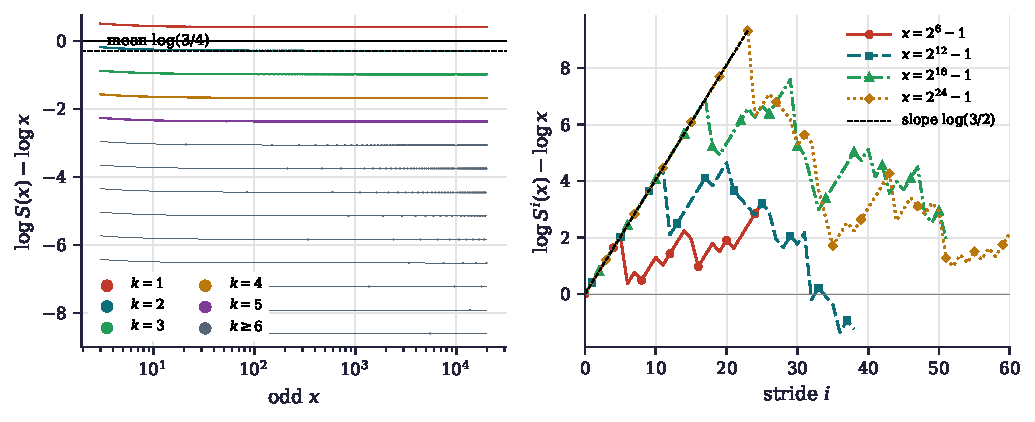
\includegraphics[width=\textwidth]{figures/ch4_stride_runs.pdf}
\caption{Left: the stride increment $\log S(x)-\log x$ for every odd
$x\le20000$, coloured by $k=\vt(3x+1)$.  Each point lies on the curve
$\log(3+1/x)-k\log2$ of its $k$ (thin lines), and only $k=1$ lies above zero; the dashed
line is the model mean $\log(3/4)$.  Right: the log trajectory
$\log S^{i}(x)-\log x$ for $x=2^{j}-1$ with $j=6,12,18,24$.  Each climbs in a
straight run of $j-1$ ascending strides, close to the black dashed line of slope
$\log(3/2)$, before the first descent (\cref{prop:ch4:chain}).}
\label{fig:ch4:runs}
\end{figure}

\section{No monotone strong Lyapunov function for a single stride}\label{sec:ch4:nolyap}

\Cref{thm:stride} already contains the first obstruction.  If half of all odd
integers ascend, then no function that increases with $x$ can decrease along
every stride.

\begin{theorem}[Impossibility of a monotone single stride strong Lyapunov function]
\label{thm:nolyapunov}
Let $W$ be a strictly increasing function from the odd positive integers to
$(0,\infty)$, and let $\rho\le1$.  Then $W(S(x))>\rho\,W(x)$ for every
$x\equiv3\pmod4$.  In particular no strictly increasing $W$ is a strict or
strong Lyapunov function\index{Lyapunov function} for $(S,\{1\})$, and the set of odd integers on which
it fails contains the residue class $3\bmod4$, which has natural density $\tfrac12$ among the odd integers; for $\rho=1$ it is exactly this class.
\end{theorem}

\begin{proof}
For $x\equiv3\pmod4$, \cref{thm:stride}(iii) gives $S(x)>x$, so
$W(S(x))>W(x)\ge\rho W(x)$.  The residue class $3\bmod4$ contains half of the
odd integers.
For $\rho=1$ the inequality $W(S(x))\le W(x)$ holds at every $x\equiv1\pmod4$ with $x\ge5$, since there $S(x)<x$ by \cref{thm:stride}(ii).
\end{proof}

The same argument covers every nondecreasing $W$ with values in $(0,\infty)$, since then $W(S(x))\ge W(x)>\rho W(x)$ on the class $x\equiv3\pmod4$ when $\rho<1$, and $W(S(x))<W(x)$ fails there when $\rho=1$; and no nonincreasing $W$ works either, since $S(5)=1<5$ gives $W(S(5))\ge W(5)$. So no monotone $W$ is a strict or strong Lyapunov function for $(S,\{1\})$.

The proof is two lines, and the theorem is correspondingly robust.  It does
not depend on the form of $W$, only on its monotonicity, and it does not
depend on any probabilistic model.  It applies to $W=\log x$, to $W=x^p$ for
every $p>0$, to $W=(\log x)^2$ on $x\ge3$, and to any composite of these with
an increasing function.  Nor is it a boundary effect: the failures are not
confined to small $x$ or to a thin set, but occupy a full residue class.

\begin{remark}[Rate of ascent]\label{rem:ch4:ascentrate}
On the ascending class the increment is
$\log(S(x)/x)=\log(3/2+1/(2x))$, which decreases to $\log(3/2)\approx0.405$
as $x\to\infty$.  So the absolute ascent per stride is bounded below by
$\log(3/2)$ uniformly, while the relative ascent
\[
  \frac{\log S(x)}{\log x}=1+\frac{\log(3/2)}{\log x}+O\Bigl(\frac{1}{x\log x}\Bigr)
\]
tends to $1$ from above.  A reparametrization $W=\phi(\log x)$ with $\phi$
increasing converts this into $W(S(x))/W(x)=\phi(\log x+\log(3/2)+o(1))/\phi(\log x)$,
which exceeds $1$ for every increasing $\phi$; no choice of $\phi$ pushes the
ratio below $1$, and the most one can arrange is that it tends to $1$, as it
does for $\phi(u)=u^2$.
\end{remark}

\begin{remark}[Monotonicity is the essential hypothesis]\label{rem:ch4:monotone}
\Cref{thm:nolyapunov} is sharp in the following sense.  If one drops
monotonicity, then by \cref{rem:ch4:exists} a strong Lyapunov function bounded
away from zero exists if and only if the conjecture is true; if it is, the function $2^{\sigma_S(x)}$ is one.
The theorem therefore draws a precise line.  Certificates that increase with the
size of $x$ are impossible; certificates\index{certificate} that see the arithmetic of $x$ are
possible in principle but are, at present, equivalent to the conjecture.  Any
viable certificate must depend on $x$ through more than its magnitude, for
instance through its residues modulo powers of $2$ and $3$, which is where
\cref{chap:parity,chap:stochastic} and \cref{chap:divergence} look for
structure.
\end{remark}

\section{Two stride compositions}\label{sec:ch4:twostride}

A natural response to \cref{thm:nolyapunov} is to look at several strides at
once.  Every ascent is followed sooner or later by a descent, and one might
hope that over two strides the descents always win.  They do not, and the
two stride case can be analysed completely.

For odd $x$ write $k_1=\vt(3x+1)$, $y=S(x)$ and $k_2=\vt(3y+1)$.  Expanding
$S(y)=(3y+1)/2^{k_2}$ gives
\begin{equation}\label{eq:ch4:twostride}
  S^{(2)}(x)=\frac{9x+3+2^{k_1}}{2^{k_1+k_2}} .
\end{equation}

\begin{lemma}[Two stride residue classes]\label{lem:ch4:tworesidue}
For integers $a,b\ge1$, the set of odd $x$ with $k_1=a$ and $k_2=b$ is a
single residue class modulo $2^{a+b+1}$.  Consequently it has natural density
$2^{-(a+b)}$ among the odd integers.
\end{lemma}

\begin{proof}
The condition $k_1=a$ says $3x+1\equiv2^a\pmod{2^{a+1}}$, and since $3$ is
invertible modulo $2^{a+1}$ this is a single class $x\equiv x_0\pmod{2^{a+1}}$.
Write $x=x_0+2^{a+1}t$.  Then $S(x)=(3x_0+1)/2^a+6t=y_0+2\cdot3t$ with $y_0$
odd.  As $t$ runs over a complete residue system modulo $2^{b}$, so does $3t$,
and hence $S(x)$ runs over all odd residues modulo $2^{b+1}$, each exactly once.
The condition $k_2=b$ selects one odd residue class of $S(x)$ modulo $2^{b+1}$,
hence one class of $t$ modulo $2^b$, hence one class of $x$ modulo $2^{a+b+1}$.
There are $2^{a+b}$ odd classes modulo $2^{a+b+1}$, which gives the density.
\end{proof}

The lemma is the two stride case of the parity vector\index{parity vector} bijection of
\cref{thm:terras}, written in the language of strides.

\begin{proposition}[Exact two stride behaviour]\label{prop:ch4:twostride}
Let $x\ge3$ be odd.
\begin{enumerate}[label=(\roman*)]
\item $S^{(2)}(x)<x$ if and only if $k_1+k_2\ge4$.
\item The odd integers with a two stride descent have natural density exactly
  $\tfrac12$ among the odd integers.
\item $\displaystyle\max_{x\ge3\text{ odd}}\bigl(\log S^{(2)}(x)-\log x\bigr)
  =\log\frac{17}{7}\approx0.8873$, attained only at $x=7$, where
  $S(7)=11$ and $S^{(2)}(7)=17$.
\end{enumerate}
\end{proposition}

\begin{proof}
Put $s=k_1+k_2\ge2$.  If $s\le3$ then $2^{k_1}\ge2$ and \eqref{eq:ch4:twostride}
gives $S^{(2)}(x)\ge(9x+5)/8>x$.  If $s\ge4$ then $2^{k_1}\le2^{s-1}$, so it
suffices to check $9x+3+2^{s-1}<2^sx$, that is $(2^s-9)x>3+2^{s-1}$.  For
$s=4$ this reads $7x>11$, true for $x\ge3$; for $s\ge5$ the left side is at
least $3(2^s-9)$ and $3\cdot2^s-27-3-2^{s-1}=\tfrac52\,2^s-30>0$.  This
proves (i).

For (ii), by (i) and \cref{lem:ch4:tworesidue} the ascending set is the union
of the classes $(k_1,k_2)\in\{(1,1),(1,2),(2,1)\}$, of total density
$2^{-2}+2^{-3}+2^{-3}=\tfrac12$.

For (iii), if $(k_1,k_2)=(1,1)$ then $S^{(2)}(x)/x=(9x+5)/(4x)$, which
decreases in $x$.  The condition $k_1=1$ means $x\equiv3\pmod4$, and then
$k_2=1$ means $(3x+1)/2\equiv3\pmod4$, that is $x\equiv7\pmod8$.  The least
such $x$ is $7$, giving the ratio $68/28=17/7$.  If $s=3$ the ratio is at most
$(9x+7)/(8x)\le34/24<17/7$, and if $s\ge4$ the ratio is below $1$.
\end{proof}

Under the Geometric$(\tfrac12)$ model the two stride increment is
$\Delta_1+\Delta_2$ with mean $2\log(3/4)\approx-0.5754$, and the probability
that $k_1+k_2\le3$ is $\tfrac14+\tfrac18+\tfrac18=\tfrac12$, so the model
reproduces part (ii) exactly.  The arithmetic agrees with it at every scale we
have examined.  Over the odd $x$ with $3\le x\le20001$ the script \texttt{ch4\_ch5\_numbers.py} (see
\cref{app:code}) finds the two stride increment negative for exactly half of
the $10000$ starting values, with mean increment $-0.574681$ against the
theoretical $2\log(3/4)=-0.575364$, and largest ascent $0.8873$ at $x=7$.
Extending the scan to all odd $x$ with $3\le x<2\times10^6$ gives a descending fraction of
$0.4999995$ and mean $-0.575359$; the residual discrepancy from $\tfrac12$ is
the edge effect of truncating the residue classes of
\cref{lem:ch4:tworesidue}.

Averaging over two strides therefore doubles the mean descent without
reducing the proportion of ascending starting points at all.  The left panel
of \cref{fig:ch4:phase} shows the same phenomenon for the two step composition
of the accelerated map\index{accelerated map}, where the split is by $x\bmod4$: the class
$x\equiv1\pmod4$ falls on the curve $\log(3/4+1/(4x))$ and the class
$x\equiv3\pmod4$ on $\log(9/4+5/(4x))$, about $0.81$ above zero.
The right panel follows whole orbits of $T$ in the phase coordinates $(\log x_n,\log x_{n+1})$: every step lands on the lower branch $\log x_{n+1}=\log x_n-\log2$ or just above the upper branch $\log x_{n+1}=\log x_n+\log(3/2)$, and the orbit of $27$, for example, takes the upper branch $41$ times and the lower one only $29$ times, yet descends, because a halving moves $\log x$ by more than an odd step does.

\begin{figure}[t]
\centering
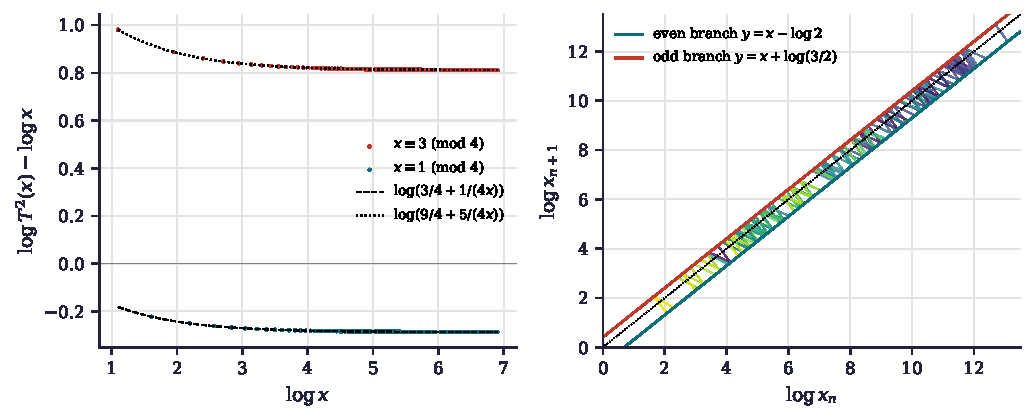
\includegraphics[width=\textwidth]{figures/ch4_phase.pdf}
\caption{Left: two step increment $\log T^{2}(x)-\log x$ of the accelerated
map for odd $x\le1000$.  The class $x\equiv1\pmod4$ descends, on the curve
$\log(3/4+1/(4x))$, which lies above its limit $\log(3/4)$; the class
$x\equiv3\pmod4$ ascends, on the curve $\log(9/4+5/(4x))$.  Right: phase
portrait in log coordinates for the accelerated orbits of $27$, $97$, $255$,
$703$ and $6171$, coloured by the fraction of the orbit elapsed.  Every step
lands on one of the two branches $\log x_{n+1}=\log x_n-\log2$ and
$\log x_{n+1}\approx\log x_n+\log(3/2)$.}
\label{fig:ch4:phase}
\end{figure}

\section{The log squared candidate}\label{sec:ch4:logsq}

A second natural response to \cref{thm:nolyapunov} is to change the potential.
Quadratic potentials are the default in optimization, and the obvious
candidate is $W(x)=(\log x)^2$.  Its behaviour illustrates, more sharply than
any other example, the difference between descent in expectation and descent
at every point.

Write $u=\log x$ and $\Delta=\log S(x)-\log x$.  Then, identically,
\begin{equation}\label{eq:ch4:logsq}
  (\log S(x))^2-(\log x)^2=(u+\Delta)^2-u^2=2u\,\Delta+\Delta^2 .
\end{equation}
Now take expectations under the stride model, in which $\Delta=\log3-k\log2$
with $k$ Geometric$(\tfrac12)$ and independent of $u$.  Then
$\E[\Delta]=\log(3/4)$ and $\Var(\Delta)=(\log2)^2\Var(k)=2(\log2)^2$, so
$\E[\Delta^2]=2(\log2)^2+(\log(3/4))^2\approx1.0437$ and
\begin{equation}\label{eq:ch4:logsqmean}
\begin{aligned}
  \E\bigl[(\log S(x))^2-(\log x)^2\bigr]
  &=2\log(3/4)\,\log x+\E[\Delta^2]\\
  &\approx-0.5754\,\log x+1.0437 .
\end{aligned}
\end{equation}
This is negative as soon as $\log x>\E[\Delta^2]/(2|\log(3/4)|)\approx1.814$,
that is for $x\ge7$, and the expected decrease grows without bound in
$\log x$.  For $J$ strides the same computation gives
$2J\log(3/4)\log x+\E[(\Delta_1+\dots+\Delta_J)^2]$, negative for
$\log x\gtrsim1.958$ when $J=2$.

One might read \eqref{eq:ch4:logsqmean} as saying that $(\log x)^2$
is a ``super Lyapunov'' function whose descent accelerates as the orbit grows.
That reading is wrong in two separate ways.

\begin{remark}[A tempting but false argument]\label{rem:ch4:logsqpitfall}
First, \eqref{eq:ch4:logsqmean} is a statement about the model, not about the
map.  For an individual $x\equiv3\pmod4$ the increment $\Delta$ is positive,
and \eqref{eq:ch4:logsq} gives $(\log S(x))^2-(\log x)^2=2u\Delta+\Delta^2>0$:
the potential increases, and by \emph{more} the larger $x$ is.  The expected
decrease and the pointwise increase both grow linearly in $\log x$; the first
averages the increase on the ascending half with the decreases on the descending half, which are larger on average.  Since
$(\log x)^2$ is increasing on $x\ge1$, \cref{thm:nolyapunov} applies to it
directly, and \cref{cor:ch4:multistride} below extends the failure to any
fixed number of strides.

Second, even in the model the growth of the absolute decrease is an artefact
of the scale of $W$.  The relative change is
\[
  \frac{\E[W(S(x))]}{W(x)}-1=\frac{2\log(3/4)}{\log x}+\frac{\E[\Delta^2]}{(\log x)^2},
\]
which tends to $0$.  Measured as a contraction factor, which is what a strong
Lyapunov function\index{Lyapunov function} requires, $(\log x)^2$ contracts \emph{less} as $x$ grows,
not more.  There is no constant $\rho<1$ with
$\E[W(S(x))]\le\rho W(x)$ for all large $x$ even in the model.
\end{remark}

The lesson generalizes.  For any potential of the form $\phi(\log x)$ with
$\phi$ smooth and increasing, a Taylor expansion gives an expected change
$\phi'(u)\log(3/4)+\tfrac12\phi''(u)\E[\Delta^2]+\cdots$, and one can choose
$\phi$ to make this negative or to make it grow.  None of these choices
touches the pointwise behaviour, which is governed by the sign of $\Delta$
alone.

\section{Multi stride certificates and chained ascents}\label{sec:ch4:multi}

The last hope for a monotone certificate\index{certificate} is to fix a number of strides $J$ and
ask for $W(S^{(J)}(x))\le\rho\,W(x)$ for all odd $x\ge3$.  For $J=2$ this
fails by \cref{prop:ch4:twostride}.  The following proposition shows that it
fails for every $J$, for an explicit and simple reason: ascending strides can
be chained to any length, and the starting points that produce long chains
are completely explicit.

\begin{proposition}[Chained ascents]\label{prop:ch4:chain}
Let $x$ be odd and write $x+1=2^{j}q$ with $q$ odd, so that $j=\vt(x+1)\ge1$.
Then for $0\le i\le j-1$,
\begin{equation}\label{eq:ch4:chain}
  S^{(i)}(x)=3^{i}\,2^{\,j-i}\,q-1 ,
\end{equation}
the first $j-1$ strides from $x$ all have $k=1$ and ascend, and the $j$th
stride has $k\ge2$ and, if $x\ge3$, descends.  In other words, the length of the initial
run of ascending strides from $x$ is exactly $\vt(x+1)-1$.
\end{proposition}

\begin{proof}
We prove \eqref{eq:ch4:chain} by induction on $i$; the case $i=0$ is the
definition of $j$ and $q$.  Suppose \eqref{eq:ch4:chain} holds for some
$i\le j-2$, and put $z=S^{(i)}(x)=3^i2^{j-i}q-1$.  Since $j-i\ge2$, $z\equiv-1
\equiv3\pmod4$, so by \cref{thm:stride}(iii) the next stride has $k=1$ and
\[
  S(z)=\frac{3z+1}{2}=\frac{3^{i+1}2^{j-i}q-2}{2}=3^{i+1}2^{\,j-i-1}q-1,
\]
which is \eqref{eq:ch4:chain} for $i+1$.  This shows that strides
$1,\dots,j-1$ have $k=1$.  For the $j$th stride, $z=S^{(j-1)}(x)=2\cdot3^{j-1}q-1$
with $3^{j-1}q$ odd, so $z\equiv1\pmod4$ and the stride has $k\ge2$, hence,
since $z\ge3$ when $x\ge3$, descends by \cref{thm:stride}(ii) (for $x=1$ the stride is $S(1)=1$).
\end{proof}

Formula \eqref{eq:ch4:chain} is the identity of \cref{rem:ch2:pitfall} written
for $S$, and it is classical: see Hercher\index{Hercher, C.}~\cite[Lemma~8]{hercher2023},
who cites Terras\index{Terras, R.}~\cite{terras1976} for it.
For example, $x=7=2^3-1$ gives $j=3$, $q=1$, and indeed $S(7)=11=3\cdot2^2-1$,
$S^{(2)}(7)=17=9\cdot2-1$, after which $S(17)=13$ descends.  The integer
$x=2^{24}-1$ climbs through $23$ consecutive ascents, multiplying by nearly
$3/2$ each time, before its first descent; the right panel of
\cref{fig:ch4:runs} shows this and three shorter chains.

\begin{corollary}[No fixed horizon monotone certificate]\label{cor:ch4:multistride}
Fix $J\ge1$, $\rho\le1$ and a strictly increasing $W$ from the odd positive
integers to $(0,\infty)$.  Then $W(S^{(J)}(x))>\rho\,W(x)$ for every odd
$x\equiv-1\pmod{2^{J+1}}$, that is for every $x=2^{J+1}q-1$ with $q\ge1$.
This set is infinite and has natural density $2^{-J}$ among the odd integers.
Moreover, along it,
\[
  \frac{S^{(J)}(x)}{x}\;\longrightarrow\;\Bigl(\frac32\Bigr)^{J}
  \qquad(q\to\infty).
\]
\end{corollary}

\begin{proof}
If $x\equiv-1\pmod{2^{J+1}}$ then $\vt(x+1)\ge J+1$, so by
\cref{prop:ch4:chain} the first $J$ strides all ascend and
$S^{(J)}(x)>x$; monotonicity of $W$ finishes the argument.  The residue class
$-1\bmod2^{J+1}$ is one of the $2^{J}$ odd classes modulo $2^{J+1}$.  For the
limit, write $x+1=2^{j}q'$ with $j\ge J+1$ and $q'$ odd; then
\eqref{eq:ch4:chain} with $i=J$ gives
$S^{(J)}(x)/x=(3^J2^{j-J}q'-1)/(2^jq'-1)$, which tends to $(3/2)^J$ as $x$
grows within the class.
\end{proof}

The corollary is the precise content of the slogan that ``chaining ascending
strides defeats every monotone multi stride certificate''.  It says more than that each
monotone fixed horizon certificate fails somewhere: it fails on a full residue class,
and on that class $\log x$ grows over the horizon by an amount
approaching $J\log(3/2)$, which is unbounded as $J$ grows.  The
horizon cannot be chosen to outrun the chains, because the chains are as long
as the $2$ adic valuation of $x+1$, and that valuation is unbounded.
As after \cref{thm:nolyapunov}, nondecreasing $W$ are covered by the same argument, and nonincreasing $W$ fail at $x=5$, since $S^{(J)}(5)=1$ for every $J\ge1$.

\begin{remark}[How the obstruction is distributed]\label{rem:ch4:distribution}
The initial run length $\vt(x+1)-1$ has, among odd $x$, natural density
$2^{-(r+1)}$ of being equal to $r$, so long chains are rare but not negligible
in any fixed proportion: a fraction $2^{-J}$ of odd integers defeats every
$J$ stride certificate that increases with $x$.  This is the same Geometric law as the halving
exponent $k$ in \cref{prop:geom}, and for the same reason; both are statements
about the $2$ adic digits of $x$.  It is also the reason the obstruction is not
merely an artefact of small numbers.  The class $x\equiv-1\pmod{2^{J+1}}$
contains integers of every size.
\end{remark}

\section{Majorization minimization for the log potential}\label{sec:ch4:mm}

We turn now from Lyapunov functions\index{Lyapunov function} to a second piece of optimization
technology, the majorization\index{majorization} minimization (MM) principle of Lange\index{Lange, K.}, Hunter\index{Hunter, D. R.} and
Yang\index{Yang, I.}~\cite{lange2000} and Hunter and Lange~\cite{hunter2004}, and ask whether
it can supply a descent certificate\index{certificate} that the direct approach cannot.  The
answer is no, but the reason is illuminating and connects back to the
martingale\index{martingale} duality of \cref{thm:martingale}.

Recall the principle.  To minimize an objective $V$, one constructs at the
current point $x_n$ a surrogate $g(\cdot\mid x_n)$ satisfying
\emph{domination}, $g(y\mid x_n)\ge V(y)$ for all $y$, and \emph{tangency},
$g(x_n\mid x_n)=V(x_n)$.  Any move that does not increase the surrogate then
does not increase the objective, since
$V(x_{n+1})\le g(x_{n+1}\mid x_n)\le g(x_n\mid x_n)=V(x_n)$.  More generally,
for any move, the change in the objective is bounded by the change in the
surrogate.

\subsection{The linear majorizer}

Take the objective to be $V(x)=\log x$, which on the positive integers is
minimized exactly at $x=1$.  Since $\log$ is concave, its tangent line at any
$x_n>0$ lies above it:
\begin{equation}\label{eq:ch4:major}
  \log y\;\le\;g(y\mid x_n):=\log x_n+\frac{y-x_n}{x_n},\qquad y>0,
\end{equation}
with equality at $y=x_n$.  Both defining properties hold, so $g$ is a
majorizer\index{majorization} in the sense of the MM literature.

\begin{remark}[A pitfall: majorizing $-\log$]\label{rem:ch4:minuslog}
It is easy to set the problem up the wrong way round.  If one takes the
objective to be $-\log x$ and asserts that its tangent line majorizes it, the
inequality is reversed: $-\log$ is convex, so its tangent lies \emph{below} it
and is a minorizer, and nothing can be concluded about descent.  The
formulation also has the wrong target, since $-\log x$ is minimized at
$x=\infty$, not at $x=1$.  With $V=\log$ as in \eqref{eq:ch4:major}, both the
direction of the inequality and the location of the minimum are correct.
\end{remark}

Domination and tangency give the following bound\index{MM algorithm}: the true objective
improves by at least as much as the surrogate.  It holds at every step, in both
parities.

\begin{proposition}[Tangent line bound for $T_0$]\label{prop:mmdescent}
For every $x\in\N$,
\[
  V(T_0(x))-V(x)\;\le\;g(T_0(x)\mid x)-g(x\mid x)
  =\begin{cases}
     -\tfrac12, & x\text{ even},\\[2pt]
     2+\tfrac1x, & x\text{ odd}.
   \end{cases}
\]
\end{proposition}

\begin{proof}
Apply \eqref{eq:ch4:major} with $x_n=x$ and $y=T_0(x)$, and use
$g(x\mid x)=V(x)$.  For even $x$ the surrogate increment is
$(x/2-x)/x=-\tfrac12$, while the true increment is $-\log2\approx-0.693$.  For
odd $x$ the surrogate increment is $(3x+1-x)/x=2+1/x$, while the true
increment is $\log(3+1/x)\le\log(10/3)\approx1.204$ for $x\ge3$.
\end{proof}

The inequality uses only domination and tangency, so it holds for any next
iterate whatever; $T_0(x)$ is not obtained by minimizing $g(\cdot\mid x)$, and
the Collatz map is not an MM iteration in the usual sense.  Worse, the bound
certifies nothing.

\begin{proposition}[The linear majorizer cannot certify descent]\label{prop:mmfails}
Under the stochastic model for the standard map\index{standard map}, in which the parities
form the renewal\index{renewal theory} chain $(B_n)$ of \cref{thm:autocorr} and a step is odd with
stationary probability $\tfrac13$, the mean surrogate increment per step of
$T_0$ is
\[
  \tfrac13\cdot2+\tfrac23\cdot\bigl(-\tfrac12\bigr)=+\tfrac13\;>\;0,
\]
up to the $O(1/x)$ term, whereas the mean true increment per step is
$\tfrac13\log3-\tfrac23\log2=\tfrac13\log(3/4)\approx-0.0959<0$.  Per Syracuse
stride, the mean surrogate increment is $+1$ and the mean true increment is
$\log(3/4)\approx-0.2877$.
\end{proposition}

\begin{proof}
The per step values follow from \cref{prop:mmdescent} and the stationary
parity frequencies.  A stride consists of one odd step followed by $k$ even
steps, so the surrogate increments summed over a stride equal
$2+1/x-k/2$, with mean $2-\E[k]/2=1$ up to $O(1/x)$; the true increment over
the stride is \eqref{eq:ch4:stride}, with mean $\log3-2\log2$ in the model.
\end{proof}

A word on levels, since three drifts are now in play.  The figure
$\tfrac13\log(3/4)$ is the drift\index{drift} per step of $T_0$; the drift per step of the
accelerated map\index{accelerated map} $T$ is $\ds=\log(\sqrt3/2)=\tfrac12\log(3/4)\approx-0.1438$;
and the drift per Syracuse stride is $\log(3/4)$.  They are the same quantity
measured against clocks that tick on average three times, twice and once per
stride.  The comparison in \cref{prop:mmfails} is between quantities measured
on the same clock, and the sign disagreement does not depend on which clock is
used.

In the model, therefore, the surrogate drifts upward while the potential
drifts downward, and iterating the majorization will never produce a descent
certificate\index{certificate}.  The reason is visible in \eqref{eq:ch4:major}: the tangent line
is an accurate upper bound only for $y$ close to $x_n$, and the odd step
multiplies by three.  At a multiplicative jump of that size the linear bound
gives $2$ where the logarithm gives $\log3\approx1.10$, an overestimate by a
factor of about $1.8$, which is more than enough to swamp the halvings.

\subsection{Why the linear surrogate sees no drift}

There is a cleaner way to say what goes wrong, which explains why no
tinkering with the linear surrogate can help.  At the level of strides, the
surrogate increment of \eqref{eq:ch4:major} is
\[
  g(S(x)\mid x)-g(x\mid x)=\frac{S(x)}{x}-1=\frac{3+1/x}{2^{k}}-1 .
\]
Under the Geometric$(\tfrac12)$ law, $\E[2^{-k}]=\sum_{j\ge1}4^{-j}=\tfrac13$,
so the mean surrogate increment per stride, computed directly at the stride
level, is
\begin{equation}\label{eq:ch4:martsurrogate}
  \E\Bigl[\frac{S(x)}{x}\Bigr]-1=\frac{3+1/x}{3}-1=\frac{1}{3x} .
\end{equation}
Up to the vanishing term $1/(3x)$, the stride ratio $S(x)/x$ has mean exactly
one: the Syracuse iterates form a multiplicative martingale\index{martingale} in the model, just
as the accelerated iterates do in \cref{thm:martingale}.  (The value $+1$ in
\cref{prop:mmfails} is larger because there the majorizer\index{majorization} is recentred at
every intermediate step, and each recentring adds a further Jensen gap\index{Jensen inequality}.)  A
linear surrogate measures the expected change of $x$ itself, which is zero to
first order, and is therefore structurally blind to the descent of $\log x$,
which is the Jensen defect
$\E[\log(S(x)/x)]-\log\E[S(x)/x]\approx\log(3/4)$.  This is the martingale
duality of \cref{chap:stochastic} seen through the MM lens: any surrogate that
is affine in $x$ inherits the drift\index{drift} of the martingale, which is nil.

\subsection{Power majorizers and the Wald root}

If the linear surrogate is too loose under multiplication, one can ask for a
surrogate that is tighter under multiplication.  A natural family is obtained
from the inequality $\log r\le(r^{p}-1)/p$, valid for $r>0$ and $p>0$ with
equality at $r=1$.  For $0<p\le1$ define
\begin{equation}\label{eq:ch4:power}
  g_p(y\mid x)=\log x+\frac{(y/x)^{p}-1}{p}.
\end{equation}
Each $g_p$ dominates $\log y$ and is tangent to it at $y=x$, so each is an MM
majorizer\index{majorization} of $V=\log$; the case $p=1$ is the linear majorizer
\eqref{eq:ch4:major}, and as $p\downarrow0$ the surrogate tends to $\log y$
itself.  Its stride increment is $((S(x)/x)^{p}-1)/p$, and its mean under the
stride model involves the moment generating function of the log increment
$\Delta=\log3-k\log2$:
\begin{equation}\label{eq:ch4:mgf}
  M(p):=\E\bigl[e^{p\Delta}\bigr]=3^{p}\sum_{j\ge1}2^{-j}2^{-pj}
  =\frac{3^{p}}{2^{1+p}-1}.
\end{equation}

\begin{proposition}[Power majorizers]\label{prop:ch4:power}
Under the stride model, the mean stride increment of the surrogate
\eqref{eq:ch4:power}, ignoring the $1/x$ correction, is $(M(p)-1)/p$, and:
\begin{enumerate}[label=(\roman*)]
\item $M(0)=M(1)=1$, and $M(p)<1$ for $0<p<1$;
\item $p\mapsto(M(p)-1)/p$ is increasing on $(0,1]$, tends to
  $\E[\Delta]=\log(3/4)$ as $p\downarrow0$, and equals $0$ at $p=1$.
\end{enumerate}
In particular every power majorizer with $0<p<1$ has strictly negative mean
surrogate increment, and the linear majorizer $p=1$ sits exactly on the
boundary.
\end{proposition}

\begin{proof}
From \eqref{eq:ch4:mgf}, $M(0)=1/(2-1)=1$ and $M(1)=3/(4-1)=1$.  A moment
generating function of a nondegenerate random variable is strictly convex, so
$M<1$ strictly between its two roots of $M=1$.  For (ii), $(M(p)-1)/p$ is the
slope of the chord of the convex function $M$ from $0$ to $p$, which is
nondecreasing in $p$ and tends to $M'(0)=\E[\Delta]$ as $p\downarrow0$; strict
convexity makes it increasing.
\end{proof}

Numerically, $M(\tfrac12)=\sqrt3/(2\sqrt2-1)\approx0.9473$, so the surrogate
$g_{1/2}$ has mean stride increment about $-0.105$, against $-0.181$ for
$p=\tfrac14$ and $-0.047$ for $p=\tfrac34$.  The family interpolates
monotonically between the true drift\index{drift} $\log(3/4)$ at $p=0$ and the martingale\index{martingale}
drift $0$ at $p=1$.  The point $p=1$ is the nonzero root of $M(p)=1$, the
\emph{Wald root} of the stride walk; it is the stride counterpart of the Wald
root $1$ of the accelerated map (\cref{thm:martingale}), and it is not a coincidence that
it falls exactly on the linear majorizer.  The equation $M(p)=1$ is the
statement that $e^{p\log x}=x^{p}$ is a martingale, and at
$p=1$ that is the martingale property of $x$ itself.  Including the exact
correction, $M_x(p)=(3+1/x)^{p}/(2^{1+p}-1)$, so $M_x(1)=1+1/(3x)$ as in
\eqref{eq:ch4:martsurrogate}, and for each $p<1$ the mean surrogate increment
is negative for all sufficiently large $x$.

Equivalently, for $0<p<1$ the function $W_p(x)=x^{p}$ is a supermartingale\index{supermartingale}
along strides in the model, $\E[W_p(S(x))]\approx M(p)\,W_p(x)$ with
$M(p)<1$: in the model it is even a geometric Foster function.

\subsection{What a multiplicatively tight majorizer would need}

\Cref{prop:ch4:power} shows that tightening the majorizer\index{majorization} under
multiplication does exactly what one would hope at the level of the model: as
soon as the surrogate curves below the tangent line, its mean increment turns
negative.  It also shows what it cannot do.  Every $g_p$ is an increasing
function of $y$, so the surrogate increment is positive whenever $S(x)>x$,
that is on the whole residue class $x\equiv3\pmod4$; and $W_p=x^{p}$ is
strictly increasing, so \cref{thm:nolyapunov} and \cref{cor:ch4:multistride}
apply to it without change.  A majorizer that certified descent pointwise
would have to satisfy three requirements at once.
\begin{enumerate}[label=(\alph*)]
\item It must dominate $\log$ and be tangent to it, so that surrogate descent
  implies true descent.
\item It must be tight enough under multiplication that its drift in the
  model is negative; by \cref{prop:ch4:power} this means curving below the
  linear majorizer, as $g_p$ does for $p<1$.
\item Its increment must be negative at every odd $x$, including those with
  $k=1$, and over every horizon, including the chains of
  \cref{prop:ch4:chain}.
\end{enumerate}
Requirements (a) and (b) are compatible and are met by the power family.
Requirement (c) is incompatible with (a) for every surrogate, because on the
ascending class $\log S(x)>\log x$, and domination and tangency then force the
surrogate increment up to at least $\log S(x)-\log x>0$, as in
\cref{prop:mmdescent}.  No majorizer of $\log$ can meet all three; a certificate
of this kind would have to majorize a potential other than $\log x$, one that
depends on the arithmetic of $x$ and not merely on its magnitude, and by
\cref{rem:ch4:monotone} constructing one is, as far as anyone
knows, as hard as the conjecture.  We do not know of one, and we regard the
search for an MM certificate\index{certificate} of this kind as a reformulation of the problem
rather than a route around it.

\section*{Notes}

Lyapunov's 1892 memoir on the stability of motion, available in English translation~\cite{lyapunov1992}, is the origin of the method;
for discrete systems, including the invariance principle, see
LaSalle~\cite{lasalle1986}.  Foster's criterion\index{Foster criterion} appeared in
Foster~\cite{foster1953}; the systematic theory of drift\index{drift} conditions, including
geometric drift and its relation to geometric ergodicity, is in Meyn and
Tweedie~\cite{meyn1993}, whose second edition (Cambridge University Press,
2009) adds a new prologue and, by Meyn, commentary and an epilogue on later developments.  The equivalence of
the conjecture with finiteness of all stopping times\index{stopping time}
(\cref{prop:ch4:eventual}) is folklore and is implicit in
Terras\index{Terras, R.}~\cite{terras1976}; see also the survey of Lagarias\index{Lagarias, J. C.}~\cite{lagarias1985}
and the collection~\cite{lagarias2010}.  The stride descent theorem is a direct
computation from the definition of $S$, and the impossibility of a monotone
certificate\index{certificate} at any fixed stride depth follows in one line from the chained
ascent formula (\cref{prop:ch4:chain}), which is the classical identity
$T^{(J)}(a2^{J}-1)=a3^{J}-1$ for the accelerated map written for $S$; see
Hercher\index{Hercher, C.}~\cite[Lemma~8]{hercher2023}, who cites Terras~\cite{terras1976} for it.
The observation that $x\equiv-1\pmod{2^{j}}$ produces long ascending runs
appears in many expositions of the Terras parity vector\index{parity vector}.  The exact two
stride analysis (\cref{prop:ch4:twostride}) and the power majorizer\index{majorization}s
(\cref{prop:ch4:power}) are presented here for the first time in this form.
For the MM principle see Lange, Hunter and Yang~\cite{lange2000}, Hunter and
Lange~\cite{hunter2004} and, for incremental versions,
Mairal\index{Mairal, J.}~\cite{mairal2015}.  The role of Wald's identity\index{Wald identity}, of the overshoot (\cref{prop:ch4:passage}) and of the root of the
moment generating function in random walks with negative drift is standard;
in the Collatz setting the corresponding computations for the accelerated map\index{accelerated map}
are in \cref{chap:stochastic}.

\section*{Exercises}

\begin{exercise}
Show that for odd $x$ and $j\ge1$, $\vt(3x+1)=j$ exactly when $x$ lies in a
single residue class modulo $2^{j+1}$, and find this class for $j=1,2,3,4$.
Deduce that $\vt(3x+1)=1$ if and only if $x\equiv3\pmod4$.
\end{exercise}

\begin{exercise}
Prove \eqref{eq:ch4:twostride}. The two stride ascending set of
\cref{prop:ch4:twostride} is a union of residue classes modulo $16$; find
them, and check that there are exactly four of them among
the eight odd classes.
\end{exercise}

\begin{exercise}
Let $x\equiv3\pmod4$ and put $j=\vt(x+1)$, so that $j\ge2$.  Use \cref{prop:ch4:chain} to show that
$\log S^{(j-1)}(x)-\log x>(j-1)\log(3/2)$.  Conclude that for every $B>0$
there is an odd $x$ and a number of strides $J$ with
$\log S^{(J)}(x)-\log x>B$, so that no bound on the cumulative ascent holds
uniformly in the horizon.
\end{exercise}

\begin{exercise}
Using the Geometric$(\tfrac12)$ law, compute $M(p)=\E[e^{p\Delta}]$ for the
stride increment and verify \eqref{eq:ch4:mgf}.  Repeat the computation for
the accelerated map\index{accelerated map} with the Bernoulli$(\tfrac12)$ model of
\cref{thm:martingale}, and show that its nonzero Wald root is also $1$.
Explain why both roots must equal $1$ whenever the iterates form a
multiplicative martingale\index{martingale}.
\end{exercise}

\begin{exercise}\label{ex:ch4:passage}
In the stride model, let $\tau$ be the first stride at which $\log x\le0$, and $O\ge0$ the overshoot below $0$ at time $\tau$, as in \cref{prop:ch4:passage}. Explain where the optional stopping argument in the proof of \cref{thm:ch4:foster} breaks down for $V=\log x$, and why the bound $\log x_0/|\log(3/4)|$ that it would give is never valid. For $s\ge0$ let $V_s=\log x+s$ when $\log x>0$ and $V_s=0$ when $\log x\le0$. Show that $V_s$ satisfies the drift condition with $\varepsilon=|\log(3/4)|$ at every $x$ with $\log x>0$ if and only if $s\ge2\log2$, and deduce from the hitting time bound that $\E_{x_0}[\tau]\le(\log x_0+2\log2)/|\log(3/4)|$, the upper half of \eqref{eq:ch4:fosterbound} with $\le$ in place of $<$.
\end{exercise}

\begin{exercise}
For the accelerated map $T$ and the linear majorizer\index{majorization} \eqref{eq:ch4:major},
show that the surrogate increment is $\tfrac12+\tfrac1{2x}$ for odd $x$ and
$-\tfrac12$ for even $x$, so that under the Bernoulli$(\tfrac12)$ model its
mean is $1/(4x)$.  Relate this to the martingale property in
\cref{thm:martingale}.
\end{exercise}
